% ============================ Enrico Ribiani 16-03-2021 ====================================================================
% Base per i documenti  
\documentclass[12pt]{article}
% ------------ pacchetti necessari ----------------
\usepackage[a4paper, total={6in, 8in},margin=1in]{geometry} % formattazione decente della pagina
\usepackage{graphicx}                            % need for figure
\usepackage{amsmath}
\usepackage{amsfonts}                            % if you want the fonts
\usepackage{amssymb}                             % if you want extra symbols
\usepackage{graphicx}  
\renewcommand{\figurename}{Figura}  
\renewcommand{\contentsname}{Indice}                        % need for figures
\usepackage{mathptmx}
\usepackage{float}                               % serve per mettere tabelle e immagini dove si vuole 
\usepackage[utf8]{inputenc}
\usepackage{textcomp}
\usepackage[hang,flushmargin,bottom]{footmisc}   % footnote format
\usepackage{fancyhdr, lastpage}
\usepackage{titlesec}
\usepackage[table,dvipsnames]{xcolor}
%\pagestyle{fancy}
%\renewcommand{\headrulewidth}{0pt}
%\renewcommand*\contentsname{Indice}
\titleformat{\section}{\normalsize\bfseries}{\thesection.}{1em}{}	% required for heading numbering style
\titleformat*{\section}{\Large\bfseries}
\titleformat*{\subsection}{\large\bfseries}
%\usepackage{siunitx}
%\usepackage{tikz}
\usepackage{circuitikz}
%\usepackage[siunitx]{circuitikz}
\usepackage{multirow}
\usepackage{tikz}
\usepackage{amsmath}
\usetikzlibrary{angles,quotes}
\usepackage{placeins}
\usepackage{multirow}
%===================links=================
\usepackage{hyperref}
\hypersetup{
    colorlinks=true,
    linkcolor=Sepia,
    filecolor=Green,      
    urlcolor=Cyan,
    pdftitle={SAMPLE},
    pdfpagemode=FullScreen,
    }
%===================inizio pagina del titolo=================
\begin{document}
    \begin{titlepage}
    \begin{center}
% ------------------ inizio immagine logo ----------
\begin{figure}
    \centering
    
\includegraphics{~/varie/logo.png}
    \label{fig:logo}
\end{figure}
% ------------------ fine immagine logo ----------
% ------------------ fine immagine logo ----------
-------------------------------------------------------------------------------------\\
\vspace{2\baselineskip}
\large Enrico Ribiani\\
\large 4AUB\\
\vfill

\Huge{\textbf{Esperienza laboratoriale bipolo ohmico-capacitivo-induttivo serie}}\\
\vfill

\LARGE{esperienza n°2}\\
\vfill
\large{19-10-2021}
\end{center}
%=============== fine pagina titolo ===============
\end{titlepage}
\tableofcontents
\vskip 1cm
\section{Scopo:Verificare il comportamento di un bipolo sperimentalmente confrontanto i valori reali con quelli teorici.}
    \subsection{Materiale}
    \begin{itemize}
        \item Breadboard
        \item Condensatore da \textit{100nF}
        \item Resistenza da \textit{2,2k$\Omega$}
        \item Induttore da \textit{47mH}
    \end{itemize}
    \subsection{Strumenti}
    \begin{itemize}
        \item Generatore di funzione
        \item Oscilloscopio
        \item Multimetro
    \end{itemize}
        \subsubsection{Schema}
        
        \begin{center}
            Il primo circuito verrà utilizzato per effettuare le misure su R, il secondo per effettuare le misure su C e il terzo per le misure su L.
        \end{center}
        \vskip 1cm
        \begin{circuitikz}[american voltages]
            \draw
                (0,0) -- (0,-0.2) node[ground]{}    
                to[vsourcesin, l_=\textit{v(t)}] (0,4)
                (0,4) to [short, *-, l=Ch1] (0,4)
                to[american resistor,  l_=R \textit{2,2k$\Omega$}, i=\textit{i(t)}] (4,4) 
                (4,4) to [inductor, *-, l=L \textit{47mH}] (4,0) %label ch2 da fixare
                to[capacitor, l=C\textit{100nF}] (0,0)
                (0,0) to [short, *-] (0,0)
                
            ;
        \end{circuitikz}
       
        \vskip 1cm

   \begin{circuitikz}[american voltages]
    \draw
        (0,0) -- (0,-0.2) node[ground]{}    
        to[vsourcesin, l_=\textit{v(t)}] (0,4)
        (0,4) to [short, *-, l=Ch1] (0,4)
        to[capacitor, l=C \textit{100nF}] (4,4) 
        (4,4) to [inductor, *-, l=L \textit{47mH}] (4,0) %label ch2 da fixare
        to[american resistor,  l_=R \textit{2,2k$\Omega$}] (0,0)
        (0,0) to [short, *-] (0,0)
    ;
\end{circuitikz}

\vskip 1cm

\begin{circuitikz}[american voltages]
 \draw
     (0,0) -- (0,-0.2) node[ground]{}    
     to[vsourcesin, l_=\textit{v(t)}] (0,4)
     (0,4) to [short, *-, l=Ch1] (0,4)
     to [inductor, *-, l=L \textit{47mH}] (4,4) 
     (4,4) to[capacitor, *-, l=C \textit{100nF}] (4,0) 
     to[american resistor,  l_=R \textit{2,2k$\Omega$}] (0,0)
     (0,0) to [short, *-] (0,0)
 ;
\end{circuitikz}


\section{Cenni teorici}
    %\subsection*{Generalità bipolo RLC}
   
    \subsection{Previsione comportamento}
    Il bipolo RLC è un circuito formato da un induttore, un resistore e un capacitore che in un aregime alternato si 
    comporta diversamente al variare della frequenza dal momento che $X_L$ e $X_C$ ne dipendono, ci sono tre scenari possibili:
    \begin{enumerate}
        \item $X_C>X_L$\\
        In questo caso il bipolo si comporterà come un bipolo RC quindi la tensione $\vec{V}$ sarà in ritardo di 90° rispetto alla corrente $\vec{I}$
        \item $X_L>X_C$\\
        In questo caso il bipolo si comporterà come un bipolo RL quindi la tensione $\vec{V}$ sarà in anticipo di 90° rispetto alla corrente $\vec{I}$
        \item $X_L$=$X_C$\\
        In questo caso il bipolo si comporterà come un bipolo puramente resistivo quindi $\vec{V}$ sarà in fase con $\vec{I}$ in quanto la parte immaginaria del 
        vettore sarà completamente nulla.
        
    \end{enumerate}
    In questa esperienza osserveremo sperimentalmente tutti i tre casi utilizzando tre diverse frequenze, mi aspetto che 
    le sinusoidi si comportino in base alla frequenza come scritto precendentemente a meno di piccole variazioni dovuti agli srumenti di 
    misura e a i vari errori.
\section{Procedimento}
   Dopo aver controllato il materiale,calcolato fr, misurato R e $R_{pind}$ che è la resistenza parassita dell'induttore abbiamo collegato il circuito al generatore
   di funzione e l'oscilloscopio, con un circuito montato abbiamo eseguito le misurazioni per tutte le frequenze prima su R, poi abbiamo collegato l'oscilloscopio ai capi
   di C e abbiamo preso le misure per tute le frequenze, idem per L.\\
   Mentre cambiavamo frequenza dal generatore d'onda abbiamo scritto le misure sulla tabella e fatto le foto dell'oscilloscopio.
   una volta misurato il valore di tensione e tempo di ritardo \textit{$t_r$} abbiamo calcolato lo sfasamento. 
   
   \vskip 1cm 
   \subsection{Foto}
    \begin{figure}[!h]
        \centering
        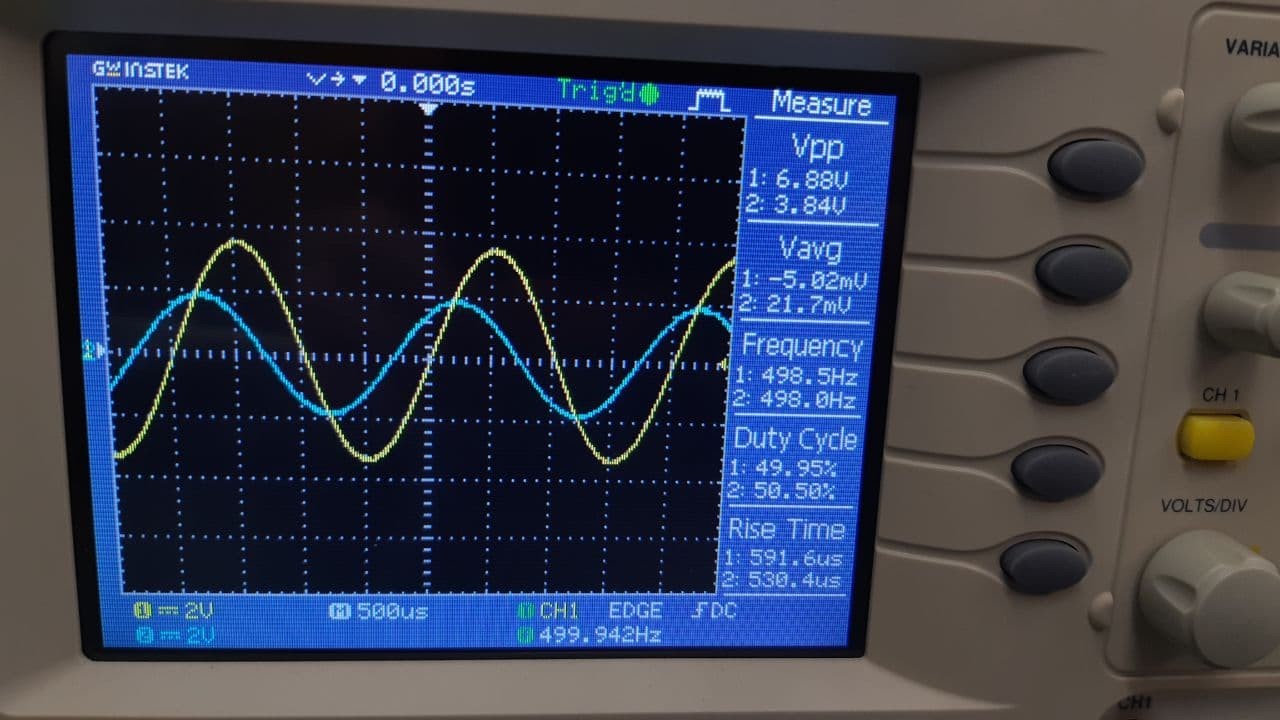
\includegraphics[scale=0.2]{media/f1vr.jpg}
        \caption{$V_R$ 500Hz}
    \end{figure}
    \begin{figure}[!h]
        \centering
        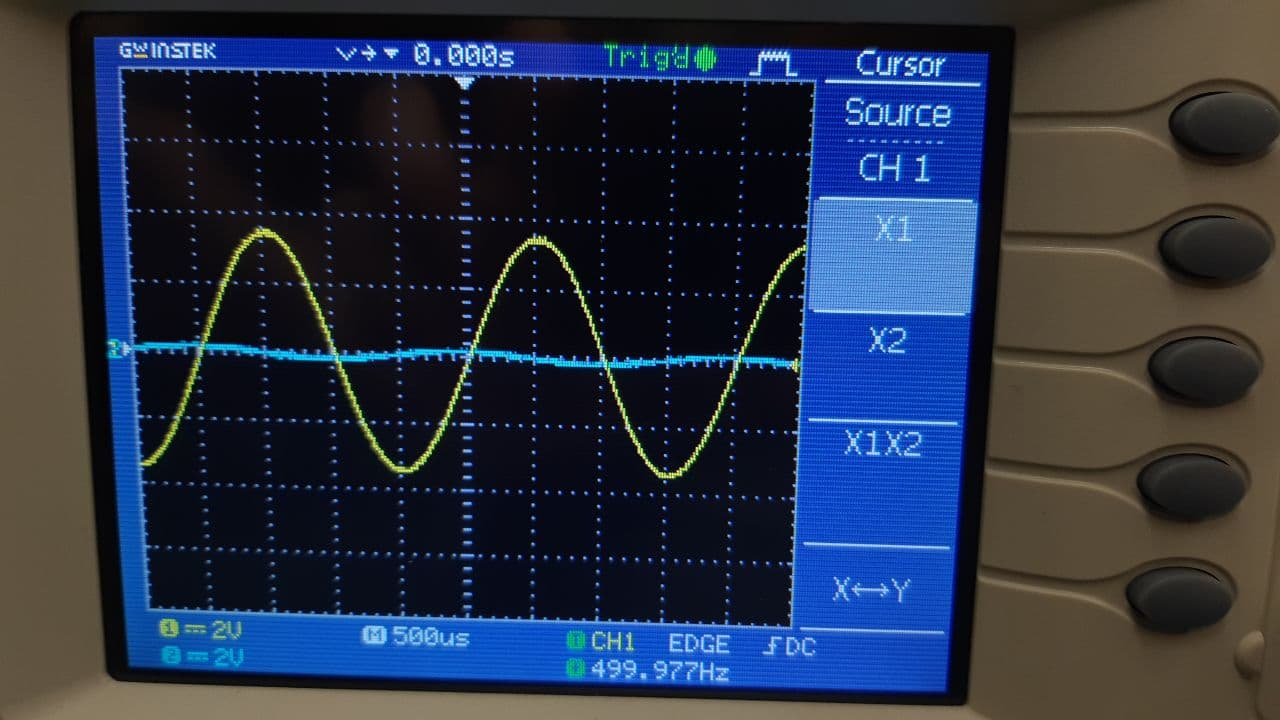
\includegraphics[scale=0.2]{media/f1vl.jpg}
        \caption{$V_L$ 500Hz}
    \end{figure}
    \begin{figure}[!h]
        \centering
        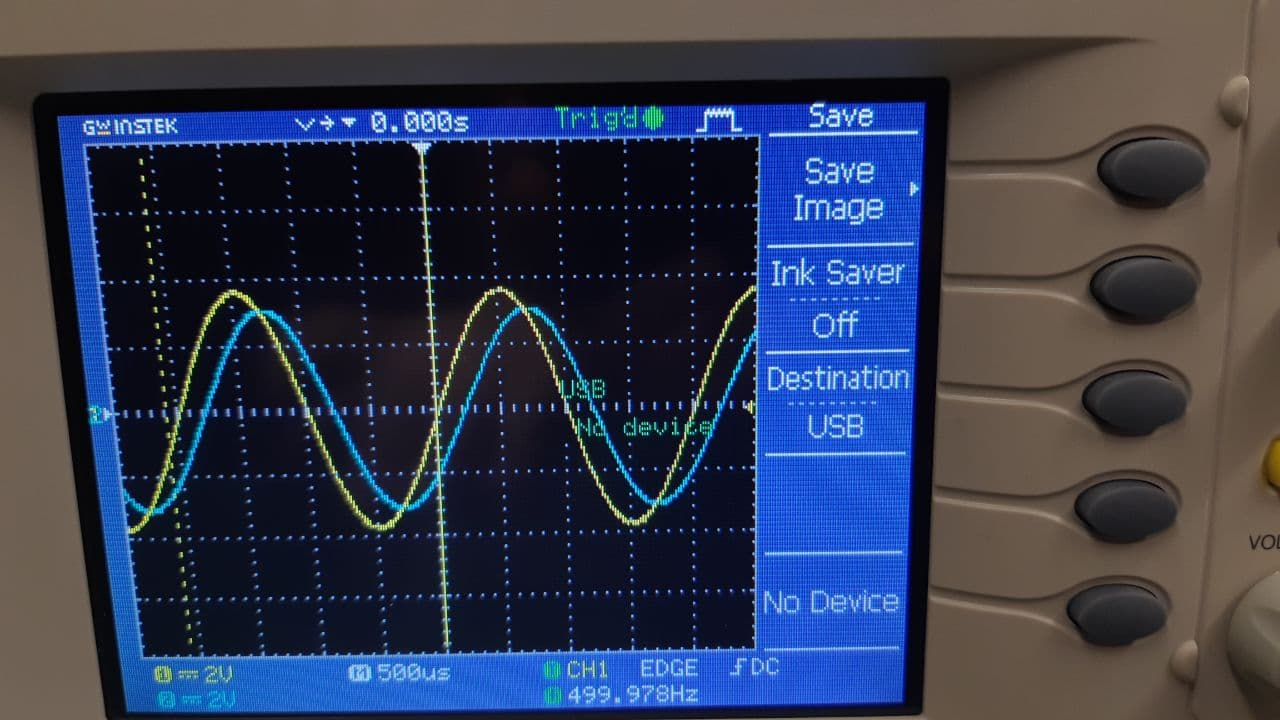
\includegraphics[scale=0.2]{media/f1vc.jpg}
        \caption{$V_C$ 500Hz}
    \end{figure}
    \begin{figure}[!h]
        \centering
        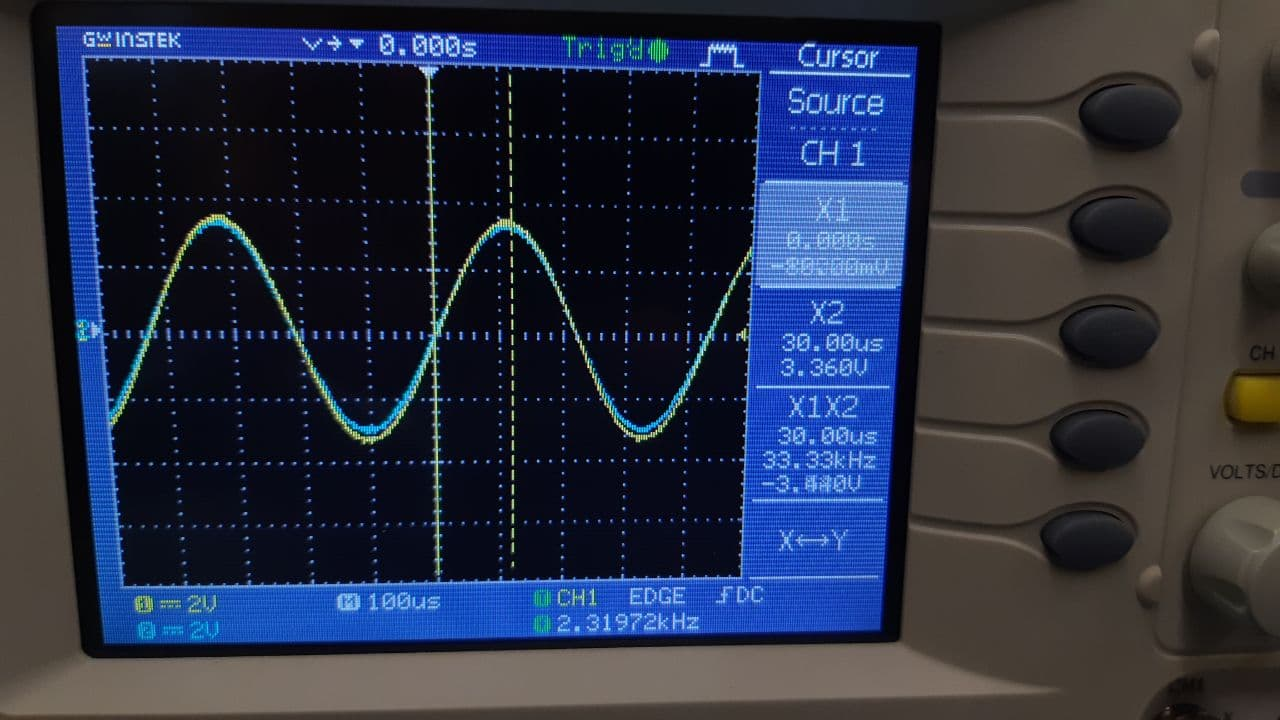
\includegraphics[scale=0.2]{media/frvr.jpg}
        \caption{$V_R$ fr}
    \end{figure}
    \begin{figure}[!h]
        \centering
        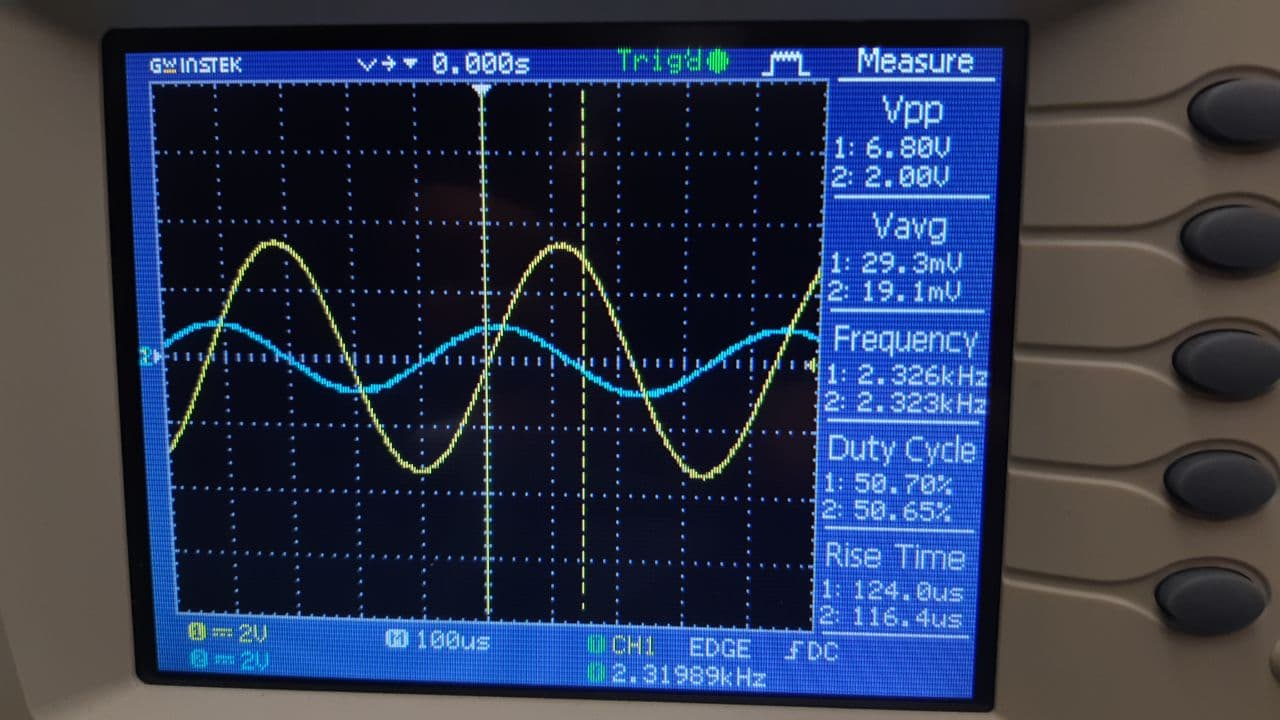
\includegraphics[scale=0.2]{media/frvl.jpg}
        \caption{$V_L$ fr}
    \end{figure}
    \begin{figure}[!h]
        \centering
        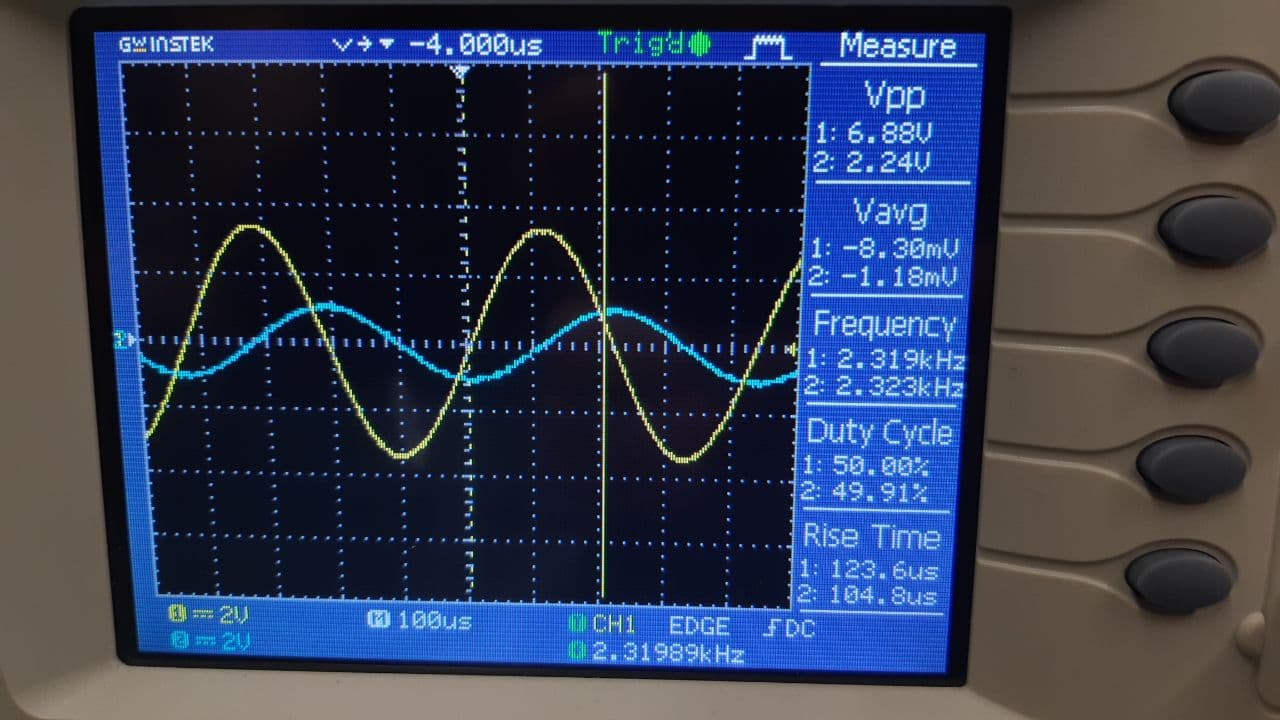
\includegraphics[scale=0.2]{media/frvc.jpg}
        \caption{$V_C$ fr}
    \end{figure}
    \begin{figure}[!h]
        \centering
        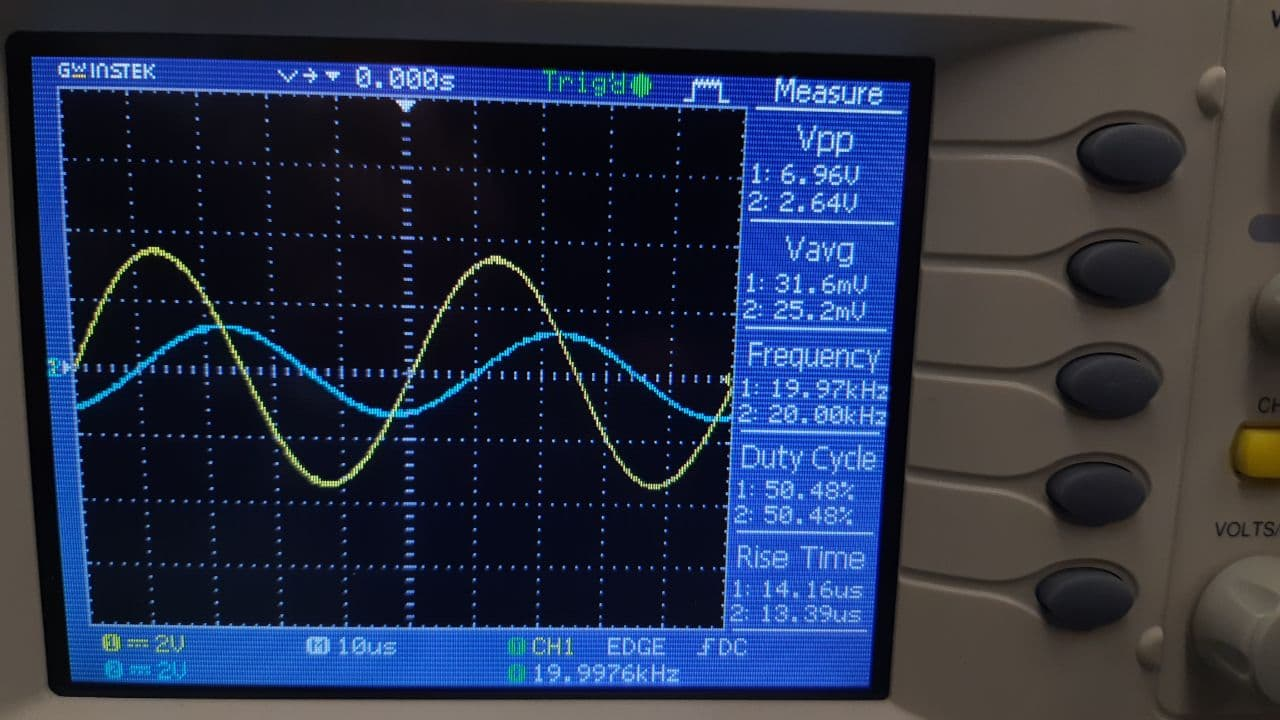
\includegraphics[scale=0.2]{media/f2vr.jpg}
        \caption{$V_R$ f=20kHz}
    \end{figure}
    \begin{figure}[!h]
        \centering
        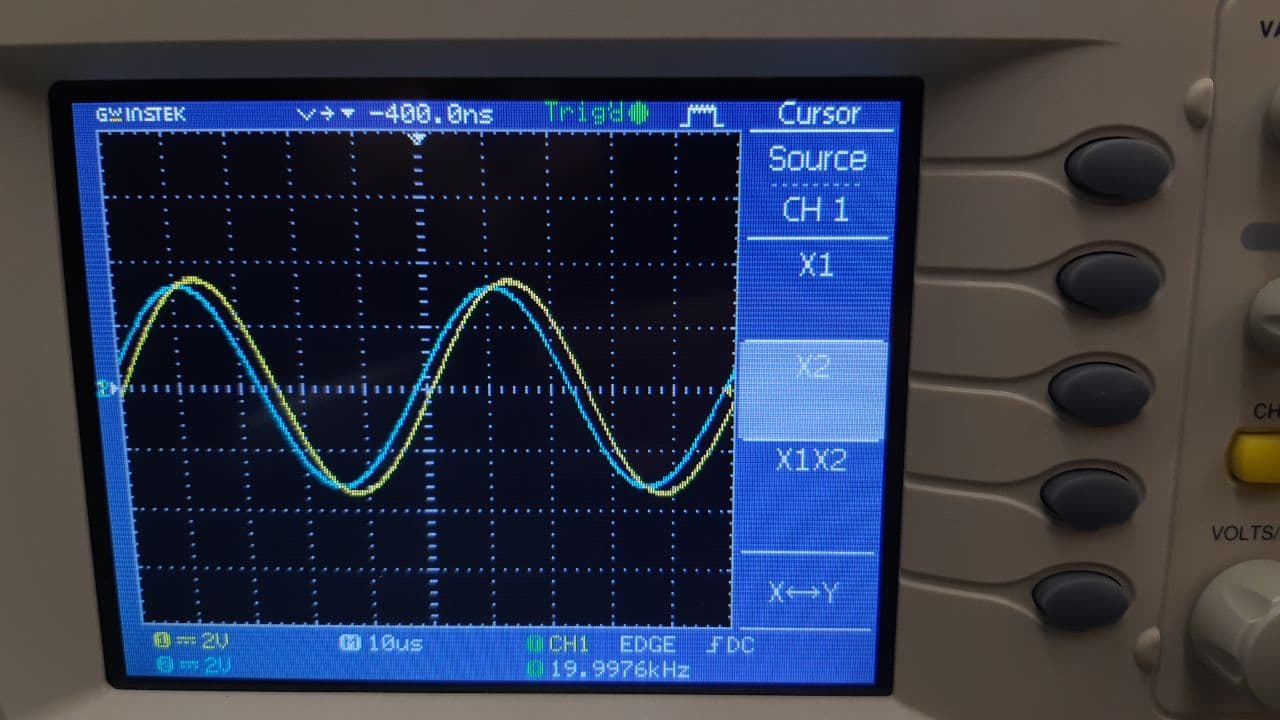
\includegraphics[scale=0.2]{media/f2vl.jpg}
        \caption{$V_L$ f=20kHz}
    \end{figure}
    \begin{figure}[!h]
        \centering
        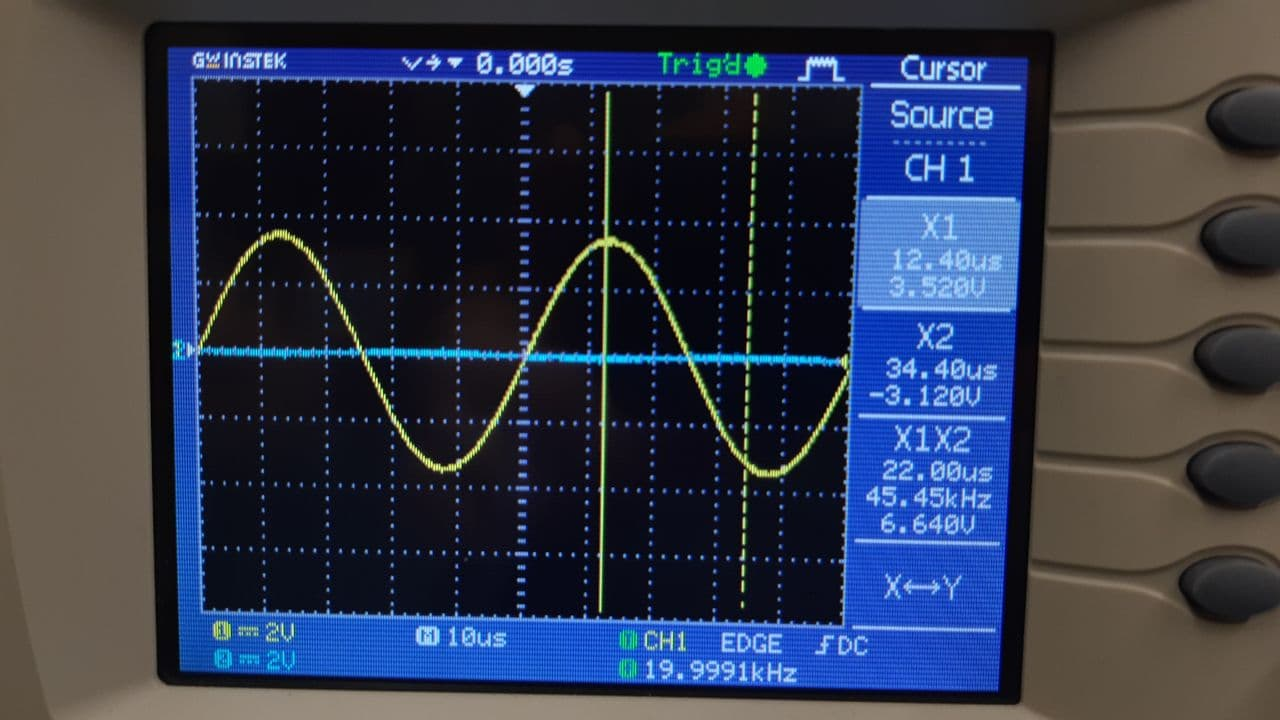
\includegraphics[scale=0.2]{media/f2vc.jpg}
        \caption{$V_C$ f=20kHz}
    \end{figure}

    \FloatBarrier
\subsection{Tabelle}    
\vspace{1cm}        

\begin{table}[!h]
        
            
        \begin{tabular}{|p{2cm}|p{2cm}|p{2cm}|p{2cm}|p{2cm}|p{2cm}|}
            \hline
            \rowcolor{BurntOrange} \textit{f}[Hz] & Comp- & $V_{pp}$ [V] & $t_r$ [$\mu$s] & $\varphi$° &  $\varphi$ rad\\
            \hline
            \rowcolor{Apricot} 500 & R & 3,48 & 300 & 54 & 0,94\\
            \hline
            \rowcolor{Apricot} 500 & L & 0,4 & 620 & 116,6 & 2,04\\
            \hline
            \rowcolor{Apricot} 500 & C & 5,84 & -216 & -39 & -0,68\\
            \hline
            \rowcolor{Peach} \textit{fr} & R & 6,40 & 30 & 5,4 & 0,1\\
            \hline
            \rowcolor{Peach} \textit{fr} & L & 2,2 & 100 & 83,52 & 1,46\\
            \hline
            \rowcolor{Peach} \textit{fr} & C & 2,2 & -102  & -85 & 1,5\\
            \hline
            \rowcolor{Apricot}  20k & R & 2,64 & -8,8 & -63,4 & 1,12\\
            \hline
            \rowcolor{Apricot} 20k & L & 6,48 & 2,8 & 20,16 &0,35\\
            \hline
            \rowcolor{Apricot} 20k & C & 0.1 & -12 & -86 & -1,5\\
            \hline
            
        \end{tabular}
        
         
    \end{table}
   
    \subsection{Calcoli}
$fr=\frac{1}{2\pi\cdot\sqrt{LC}}$\\
$\varphi:2\pi=t:T$ \\
$\varphi=\frac{2\pi \cdot t}{T}$\\
calcolo analitico:\\
$\varphi=arctg(\frac{X_L - X_C}{R})$

%il calcolo di $\varphi$ varia per ogni grandezza perché hanno tempi di ritardo diversi oltre a essere su varie frequenze\\
%\vskip 0.5cm
%$Z=\sqrt{R^2+(X_L-X_C)^2}=3038\Omega$\\
%$I=\frac{V}{Z}=\frac{2,47V}{3038\Omega}=0,8mA$\\
%$X_L=\omega L=2 \pi\cdot f \cdot L=147,8\Ohm$


\section{Conclusioni}
Osservando i risultati ottenuti possiamo notare che viene seguito il comportamento teorico del circuito a parte per lo sfasamento dato
dalla resistenza parassita dell'induttore che risulta rilevante solo quando vengono paragonati i valori teorici e quelli misurati, per quanto riguarda i 
diagrammi vettoriali esso non presenta un problema. 
Lo sfasamento pratico della tensione sulla corrente è uguale a $\varphi$ di R perhcè la tensione ai capi di R è in fase con la corrente
e dal momento che per comodità abbiamo stabilito che $\vec{V}$ è posizionato sull'asse delle X.


\subsection{Diagrammi vettoriali}
u=1V ma sono stati usati nel grafico i valori picco picco.\\
\textit{f=500Hz}   u=1V \\
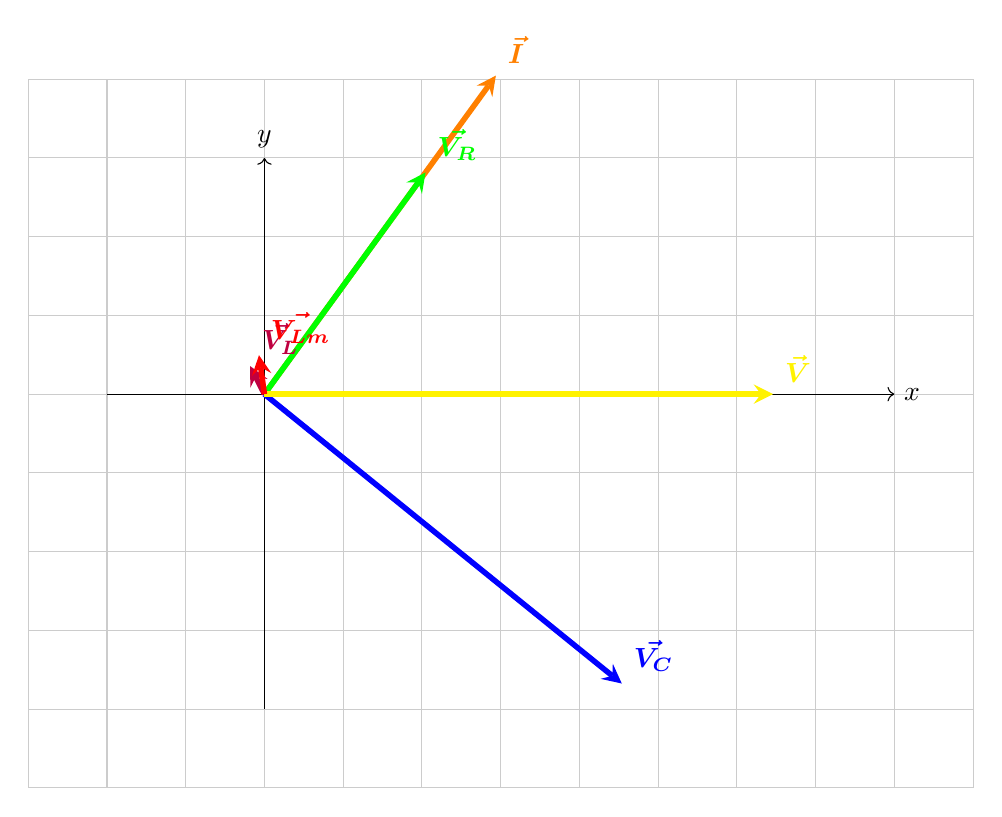
\begin{tikzpicture}
    \draw[thin,gray!40] (-3,-5) grid (9,4);
    \draw[->] (-2,0)--(8,0) node[right]{$x$};
    \draw[->] (0,-4)--(0,3) node[above]{$y$};
    \draw[line width=2pt,orange,-stealth] (0,0) -- (54:5cm) node[anchor=south west]{$\boldsymbol{\vec{I}}$};
    \draw[line width=2pt,green,-stealth] (0,0) -- (54:3.48cm) node[anchor=south west]{$\boldsymbol{\vec{V_R}}$};
    \draw[line width=2pt,blue,-stealth] (0,0) -- (-39:5.84cm) node[anchor=south west]{$\boldsymbol{\vec{V_C}}$};
    \draw[line width=2pt,purple,-stealth] (0,0) -- (117:0.4cm) node[anchor=south west]{$\boldsymbol{\vec{V_L}}$};
    \draw[line width=2pt,yellow,-stealth] (0,0) -- (0:6.46cm) node[anchor=south west]{$\boldsymbol{\vec{V}}$};
    \draw[line width=2pt,red,-stealth] (0,0) -- (98:0.5cm) node[anchor=south west]{$\boldsymbol{\vec{V_{Lm}}}$};
    
      

  \end{tikzpicture}

  \vskip 3cm

 


  \textit{fr}\\
  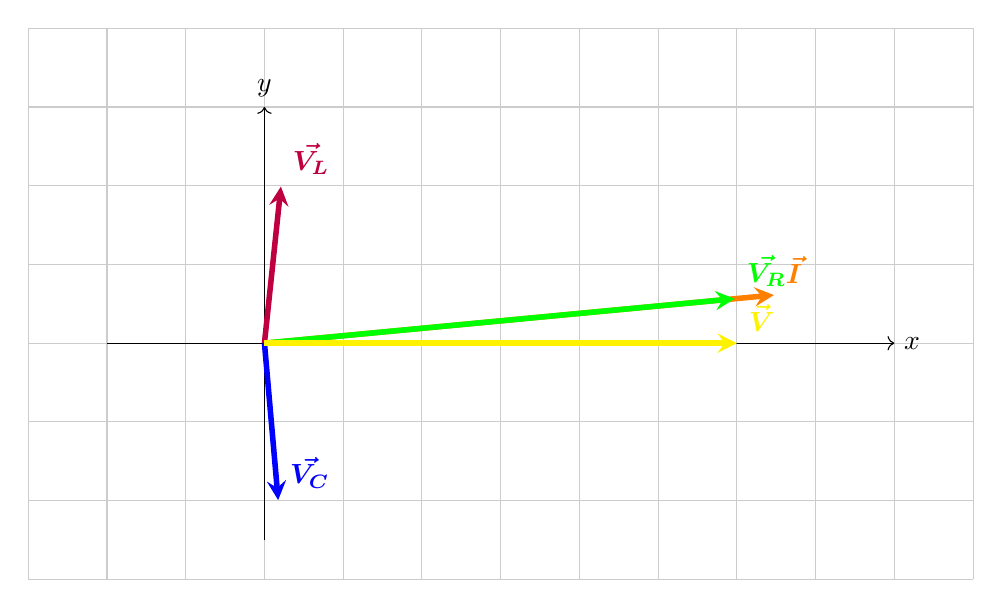
\begin{tikzpicture}
    \draw[thin,gray!40] (-3,-3) grid (9,4);
    \draw[->] (-2,0)--(8,0) node[right]{$x$};
    \draw[->] (0,-2.5)--(0,3) node[above]{$y$};
    \draw[line width=2pt,orange,-stealth] (0,0) -- (5.4:6.5cm) node[anchor=south west]{$\boldsymbol{\vec{I}}$};
    \draw[line width=2pt,green,-stealth] (0,0) -- (5.4:6cm) node[anchor=south west]{$\boldsymbol{\vec{V_R}}$};
    \draw[line width=2pt,blue,-stealth] (0,0) -- (-85:2cm) node[anchor=south west]{$\boldsymbol{\vec{V_C}}$};
    \draw[line width=2pt,purple,-stealth] (0,0) -- (84:2cm) node[anchor=south west]{$\boldsymbol{\vec{V_L}}$};
    \draw[line width=2pt,yellow,-stealth] (0,0) -- (0:6cm) node[anchor=south west]{$\boldsymbol{\vec{V}}$};
   
 
  \end{tikzpicture}
\vskip 1cm
  
  \textit{f=20kHz}\\
  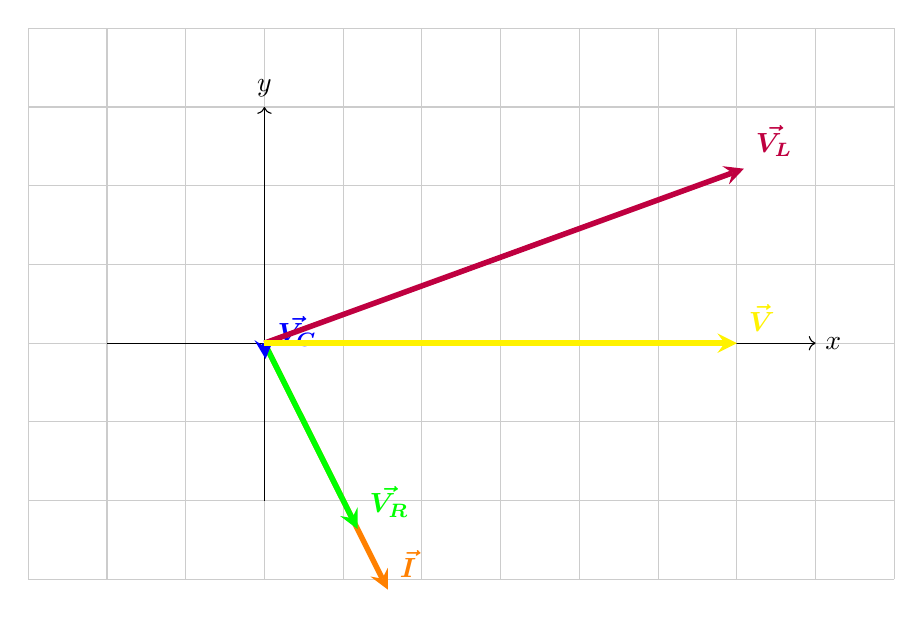
\begin{tikzpicture}
    \draw[thin,gray!40] (-3,-3) grid (8,4);
    \draw[->] (-2,0)--(7,0) node[right]{$x$};
    \draw[->] (0,-2)--(0,3) node[above]{$y$};
    \draw[line width=2pt,orange,-stealth] (0,0) -- (-63.4:3.5cm) node[anchor=south west]{$\boldsymbol{\vec{I}}$};
    \draw[line width=2pt,green,-stealth] (0,0) -- (-63.4:2.64cm) node[anchor=south west]{$\boldsymbol{\vec{V_R}}$};
    \draw[line width=2pt,blue,-stealth] (0,0) -- (-86:0.2cm) node[anchor=south west]{$\boldsymbol{\vec{V_C}}$};
    \draw[line width=2pt,purple,-stealth] (0,0) -- (20:6.48cm) node[anchor=south west]{$\boldsymbol{\vec{V_L}}$};
    \draw[line width=2pt,yellow,-stealth] (0,0) -- (0:6cm) node[anchor=south west]{$\boldsymbol{\vec{V}}$};
      
  \end{tikzpicture}
  
\end{document}
